\documentclass{article}
\usepackage{amsmath}
\usepackage{tikz}
\usetikzlibrary{calc}
\usepackage[margin=1.3cm]{geometry} % set margins


\begin{document}
{\Large 1.a)}
Para construir el segmento cuarto proporcional a los segmentos $w = 7$ cm, $z = 5$ cm y $c = 4$ cm, se pueden seguir los siguientes pasos:

\begin{enumerate}
\item Construye un triángulo rectángulo con los segmentos $w$ y $z$ como los catetos y el segmento $c$ como la hipotenusa.
\item Dibuja una altura desde el vértice del ángulo recto al lado opuesto, dividiendo así el triángulo en dos triángulos más pequeños.
\item Etiqueta la longitud de la altura como $h$.
\item Usa la relación geométrica de proporción entre los segmentos de un triángulo rectángulo para encontrar la longitud del segmento cuarto proporcional. En particular, la longitud del segmento cuarto proporcional es igual a la longitud de la hipotenusa dividida por la raíz cuadrada de 2 veces la altura:
\begin{align*}
    \text{Cuarto proporcional} &= \frac{c}{\sqrt{2h}}
\end{align*}

\item Sustituye los valores dados en la fórmula para encontrar el segmento cuarto proporcional:

\begin{align*}
    \text{Cuarto proporcional} &= \frac{4\text{ cm}}{\sqrt{2h}}
\end{align*}

\item Para encontrar la altura $h$, podemos usar el teorema de Pitágoras en uno de los triángulos más pequeños:

\begin{align*}
    h^2 &= wz \\
    h &= \sqrt{wz} = \sqrt{7\text{ cm} \cdot 5\text{ cm}} = \sqrt{35}\text{ cm}
\end{align*}

\item Sustituye la altura $h$ en la fórmula para encontrar el segmento cuarto proporcional:

\begin{align*}
    \text{Cuarto proporcional} &= \frac{4\text{ cm}}{\sqrt{2\sqrt{35}\text{ cm}}} \approx 1.41\text{ cm}
\end{align*}
\end{enumerate}

Por lo tanto, el segmento cuarto proporcional a los segmentos dados es de aproximadamente $1.41$ cm.

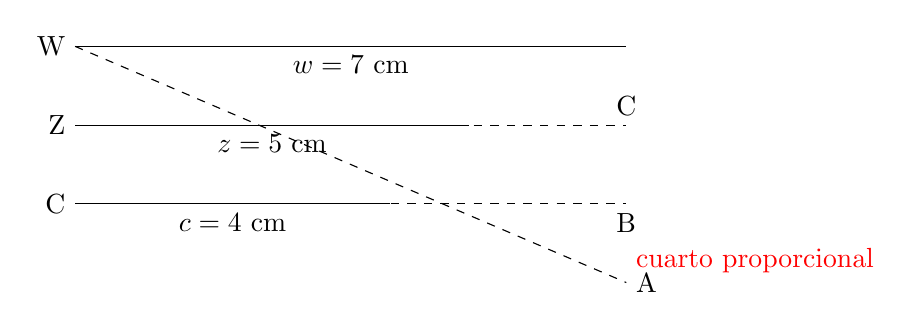
\begin{tikzpicture}
	% Segmentos w, z y c
	\draw (0,0) -- (7,0) node[midway, below] {$w=7$ cm};
	\draw (0,-1) -- (5,-1) node[midway, below] {$z=5$ cm};
	\draw (0,-2) -- (4,-2) node[midway, below] {$c=4$ cm};

	% Punto A y línea punteada
	\coordinate (A) at (7,-3);
	\draw[dashed] (0,0) -- (A);

	% Punto B y línea punteada
	\coordinate (B) at ($(0,-2)!(A)!(4,-2)$);
	\draw[dashed] (0,-2) -- (B);

	% Punto C y línea punteada
	\coordinate (C) at ($(0,-1)!(A)!(5,-1)$);
	\draw[dashed] (0,-1) -- (C);

	% Segmento cuarto proporcional
	\draw[red] (A) -- ($(B)!(A)!(C)$) node[midway, above right] {cuarto proporcional};

	% Etiquetas de los puntos
	\node at (0,0) [left] {W};
	\node at (0,-1) [left] {Z};
	\node at (0,-2) [left] {C};
	\node at (A) [right] {A};
	\node at (B) [below] {B};
	\node at (C) [above] {C};
\end{tikzpicture}
\\
{\Large 1.b)}
\\
Para construir el segmento tercero proporcional a los segmentos dados, se puede seguir los siguientes pasos:

Dibuja un segmento de línea recta con longitud "a" y etiquétalo como "AB".
Dibuja un arco de círculo con centro en "A" y radio "b". Este arco cortará la línea "AB" en un punto "C".
Dibuja otro arco de círculo con centro en "C" y radio "a". Este arco cortará la línea "AB" en un punto "D".
Dibuja un segmento de línea recta desde el punto "D" hasta el centro del arco de círculo con centro en "A". Etiqueta el punto de intersección como "E".
El segmento "DE" es el tercero proporcional a los segmentos "a" y "b".
La construcción se puede visualizar de la siguiente manera:

La demostración de que el segmento "DE" es el tercero proporcional a los segmentos "a" y "b" se puede hacer utilizando propiedades de la geometría y álgebra, pero es un poco compleja. En lugar de eso, puede verificar la solución utilizando la relación:

$a:b::b:(DE)$

donde "::" significa "es a" o "proporcional a". Esta relación se puede simplificar para obtener:

$a^2 = b(DE)$

Sustituyendo los valores dados de "a" y "b", obtenemos:

$7^2 = 5(DE)$

$49 = 5(DE)$

$DE = \frac{49}{5} = 9.8\text{ cm}$

Por lo tanto, el segmento tercero proporcional a los segmentos "a" y "b" es de aproximadamente 9.8 cm.
\\
{\Large 1.c)}
\\
Para dividir un segmento de 13 cm en 5 segmentos iguales, se puede utilizar la siguiente fórmula:

\begin{align*}
\text{Longitud de cada segmento} &= \frac{\text{Longitud total}}{\text{Número de segmentos}} \
&= \frac{13\text{ cm}}{5} \
&= 2.6\text{ cm}
\end{align*}

Por lo tanto, cada uno de los 5 segmentos iguales tiene una longitud de 2.6 cm.
\\
{\Large 1.d)}
\\
Para dividir el segmento de $11$ cm en $5$ segmentos proporcionales a los segmentos dados, podemos utilizar la proporción:

$$\frac{2\text{ cm}}{17} : \frac{3.5\text{ cm}}{17} : \frac{4\text{ cm}}{17} : \frac{1.5\text{ cm}}{17} : \frac{6\text{ cm}}{17} = \frac{x}{11\text{ cm}} : \frac{x}{11\text{ cm}} : \frac{x}{11\text{ cm}} : \frac{x}{11\text{ cm}} : \frac{x}{11\text{ cm}}$$

Donde $x$ es la medida de cada uno de los $5$ segmentos proporcionales.

Para encontrar la medida de cada uno de los $5$ segmentos proporcionales, podemos multiplicar cada término en el lado derecho de la proporción por $11$ cm:

$$\begin{aligned}
	x &= \frac{2\text{ cm}}{17} \times 11\text{ cm} = \frac{22}{17}\text{ cm} \approx 1.29\text{ cm} \\
	x &= \frac{3.5\text{ cm}}{17} \times 11\text{ cm} = \frac{38.5}{17}\text{ cm} \approx 2.26\text{ cm} \\
	x &= \frac{4\text{ cm}}{17} \times 11\text{ cm} = \frac{44}{17}\text{ cm} \approx 2.59\text{ cm} \\
	x &= \frac{1.5\text{ cm}}{17} \times 11\text{ cm} = \frac{16.5}{17}\text{ cm} \approx 0.97\text{ cm} \\
	x &= \frac{6\text{ cm}}{17} \times 11\text{ cm} = \frac{132}{17}\text{ cm} \approx 7.76\text{ cm}
\end{aligned}$$

Por lo tanto, los $5$ segmentos proporcionales miden aproximadamente:

- $1.29$ cm
- $2.26$ cm
- $2.59$ cm
- $0.97$ cm
- $7.76$ cm
\\
{\Large 1.e)}
\\
Para dividir el segmento AB de $7$ cm en dos partes proporcionales a los segmentos de $5$ cm y $4$ cm, podemos utilizar la proporción:

$$5\text{ cm} : 4\text{ cm} = x : (7 - x)$$

Donde $x$ es la longitud de uno de los dos segmentos proporcionales.

Podemos resolver esta proporción para obtener el valor de $x$:

$$\begin{aligned}
	5\text{ cm} : 4\text{ cm} &= x : (7 - x) \\
	5(7 - x) &= 4x \\
	35 - 5x &= 4x \\
	9x &= 35 \\
	x &= \frac{35}{9}\text{ cm} \approx 3.89\text{ cm}
\end{aligned}$$

Por lo tanto, el segmento AB puede ser dividido en dos segmentos proporcionales de longitud:

- $x = \frac{35}{9}\text{ cm} \approx 3.89\text{ cm}$
- $7 - x = \frac{38}{9}\text{ cm} \approx 3.11\text{ cm}$
\\
{\Large 1.f)}
\\
Para dividir el segmento de $13$ cm en dos partes cuya razón sea $3/4$, podemos utilizar la proporción:

$$3 : 4 = x : (13 - x)$$

Donde $x$ es la longitud de una de las dos partes proporcionales.

Podemos resolver esta proporción para obtener el valor de $x$:

$$\begin{aligned}
	3 : 4 &= x : (13 - x) \\
	4x &= 3(13 - x) \\
	4x &= 39 - 3x \\
	7x &= 39 \\
	x &= \frac{39}{7}\text{ cm} \approx 5.57\text{ cm}
\end{aligned}$$

Por lo tanto, el segmento de $13$ cm se puede dividir en dos partes proporcionales de longitud:

- $x = \frac{39}{7}\text{ cm} \approx 5.57\text{ cm}$
- $13 - x = \frac{64}{7}\text{ cm} \approx 7.43\text{ cm}$
\\
{\Large 3.}
\\
La homotecia es una transformación geométrica que consiste en ampliar o reducir una figura en relación a un punto fijo llamado centro de homotecia y por un factor de escala constante llamado razón de homotecia.

En otras palabras, la homotecia es una transformación que mantiene la forma de una figura, pero cambia su tamaño. La figura original y su homóloga tienen la misma forma, pero una es una versión ampliada o reducida de la otra.

En una homotecia, todos los puntos de la figura original se mueven a lo largo de una recta que pasa por el centro de homotecia. Los puntos en la recta que pasa por el centro de homotecia no se mueven, ya que la razón de homotecia es constante.

La homotecia se utiliza en muchos campos de la matemática y la física, como la geometría, la trigonometría, la óptica y la mecánica. Se utiliza para modelar situaciones en las que una figura se transforma cambiando su tamaño, como en la ampliación o reducción de imágenes, la proyección de mapas y la reflexión de luz.
\\
{\Large 4. a)}
\\
Para identificar el centro de homotecia y la razón de homotecia de una transformación homotética, es necesario conocer dos figuras homólogas (es decir, dos figuras con la misma forma pero diferente tamaño) que se relacionan mediante la homotecia.

Por lo tanto, sin tener información adicional, no es posible determinar el centro de homotecia y la razón de homotecia de una transformación homotética.

En general, el centro de homotecia es el punto que se mantiene fijo durante la transformación homotética, y la razón de homotecia es el factor de escala que se aplica a las dimensiones de la figura original para obtener la figura homóloga. Ambos parámetros dependen de las figuras específicas que se están considerando.

Sin embargo, si tienes una figura original y su figura homóloga, es posible encontrar el centro de homotecia y la razón de homotecia utilizando la siguiente fórmula:

$$\text{Razón de homotecia} = \frac{\text{Distancia entre el centro de homotecia y la imagen}}{\text{Distancia entre el centro de homotecia y el objeto original}}$$

El centro de homotecia es el punto donde se intersectan las rectas que conectan cada par de puntos homólogos. La razón de homotecia se puede encontrar midiendo la distancia entre el centro de homotecia y un punto homólogo, y dividiendo ese valor por la distancia correspondiente entre el centro de homotecia y el punto homólogo correspondiente en la figura original.
\\
\\
{\Large 5.}
% Trapecio isósceles ABMC
\begin{tikzpicture}
	\draw (0,0) -- (4,0) -- (2,3) -- (-2,3) -- cycle;
	\node at (0,0) [below] {B};
	\node at (4,0) [below] {M};
	\node at (2,3) [above] {C};
	\node at (-2,3) [above] {A};
\end{tikzpicture}

% Composición de transformaciones H(C, 2) o S_A
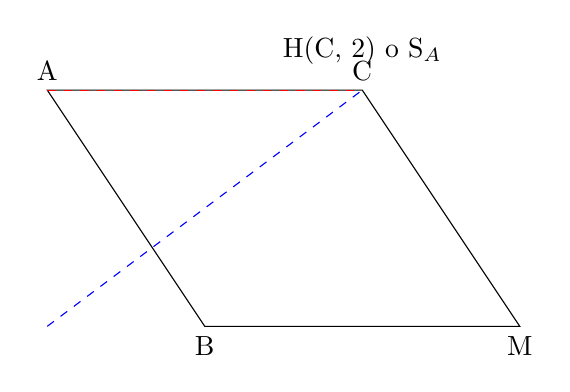
\begin{tikzpicture}
	\draw (0,0) -- (4,0) -- (2,3) -- (-2,3) -- cycle;
	\draw[red, dashed] (-2,3) -- (2,3);
	\draw[blue, dashed] (-2,0) -- (2,3);
	\node at (0,0) [below] {B};
	\node at (4,0) [below] {M};
	\node at (2,3) [above] {C};
	\node at (-2,3) [above] {A};
	\node at (2,3.5) {H(C, 2) o S$_A$};
\end{tikzpicture}

% Composición de transformaciones Se o H(A, - 1/2)
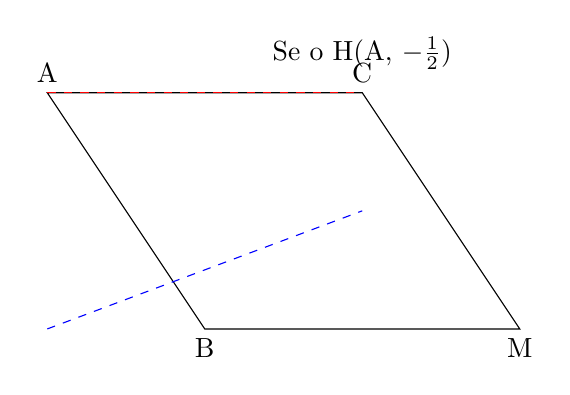
\begin{tikzpicture}
	\draw (0,0) -- (4,0) -- (2,3) -- (-2,3) -- cycle;
	\draw[red, dashed] (-2,3) -- (2,3);
	\draw[blue, dashed] (-2,0) -- (2,1.5);
	\node at (0,0) [below] {B};
	\node at (4,0) [below] {M};
	\node at (2,3) [above] {C};
	\node at (-2,3) [above] {A};
	\node at (2,3.5) {Se o H(A, $-\frac{1}{2}$)};
\end{tikzpicture}

% Composición de transformaciones T^v o H(B, -2)
\begin{tikzpicture}
	\draw (0,0) -- (4,0) -- (2,3) -- (-2,3) -- cycle;
	\draw[red, dashed] (-2,3) -- (2,3);
	\draw[blue, dashed] (0,3) -- (4,-3);
	\node at (0,0) [below] {B};
	\node at (4,0) [below] {M};
	\node at (2,3) [above] {C};
	\node at (-2,3) [above] {A};
	\node at (2,3.5) {T$^v$ o H(B, $-2$)};
\end{tikzpicture}
\\
{\Large 6.}
\\
\\
\begin{tikzpicture}
% Trapecio isósceles ABMC
\draw (0,0) -- (4,0) -- (2,3) -- (-2,3) -- cycle;
\node at (0,0) [below] {B};
\node at (4,0) [below] {M};
\node at (2,3) [above] {C};
\node at (-2,3) [above] {A};
\end{tikzpicture}

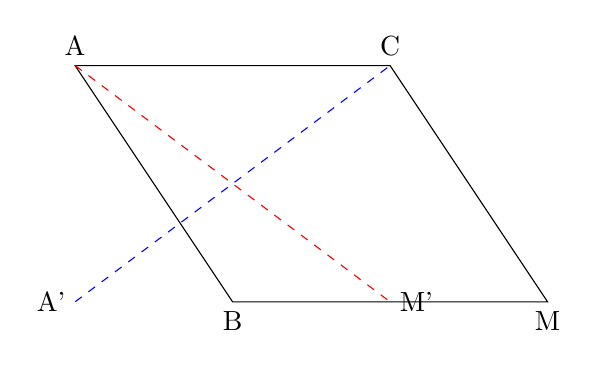
\begin{tikzpicture}
% Composición de transformaciones H(C, 2) o S_A
\draw (9,0) -- (13,0) -- (11,3) -- (7,3) -- cycle;
\draw[red, dashed] (7,3) -- (11,0);
\draw[blue, dashed] (7,0) -- (11,3);
\node at (9,0) [below] {B};
\node at (13,0) [below] {M};
\node at (11,3) [above] {C};
\node at (7,3) [above] {A};
\node at (11,0) [right] {M'};
\node at (7,0) [left] {A'};
\end{tikzpicture}

% Composición de transformaciones Se o H(A, - 1/2)
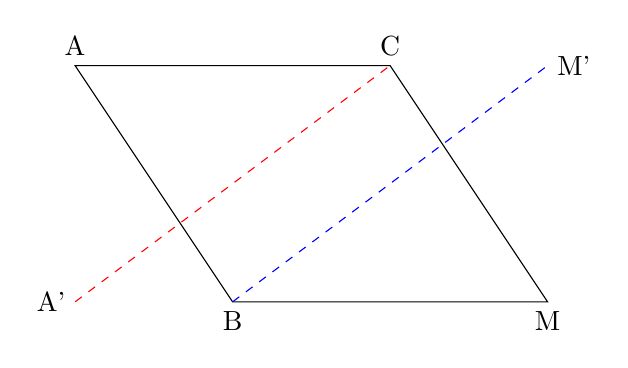
\begin{tikzpicture}
\draw (18,0) -- (22,0) -- (20,3) -- (16,3) -- cycle;
\draw[red, dashed] (16,0) -- (20,3);
\draw[blue, dashed] (18,0) -- (22,3);
\node at (18,0) [below] {B};
\node at (22,0) [below] {M};
\node at (20,3) [above] {C};
\node at (16,3) [above] {A};
\node at (22,3) [right] {M'};
\node at (16,0) [left] {A'};
\end{tikzpicture}

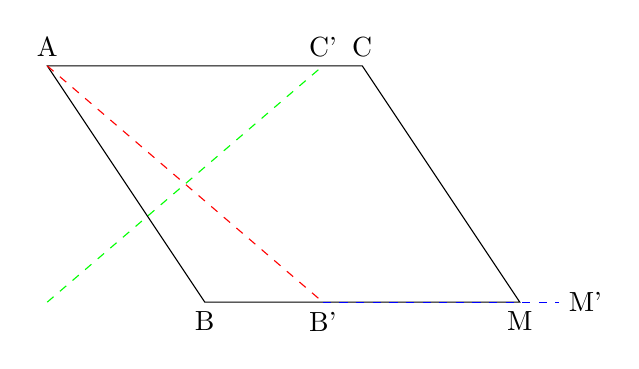
\begin{tikzpicture}
% Composición de transformaciones T^v o H(B, -2)
\draw (27,0) -- (31,0) -- (29,3) -- (25,3) -- cycle;
\draw[red, dashed] (25,3) -- (28.5,0);
\draw[blue, dashed] (28.5,0) -- (31.5,0);
\draw[green, dashed] (25,0) -- (28.5,3);
\node at (27,0) [below] {B};
\node at (31,0) [below] {M};
\node at (29,3) [above] {C};
\node at (25,3) [above] {A};
\node at (31.5,0) [right] {M'};
\node at (28.5,3) [above] {C'};
\node at (28.5,0) [below] {B'};
\end{tikzpicture}

\begin{tikzpicture}
% Composición de transformaciones H(C', 1/2) o G_{A,-80}
\draw (0,-5) -- (4,-5) -- (2,-2) -- (-2,-2) -- cycle;
\draw[red, dashed] (2,-2) -- (-1.41, -0.59);
\draw[blue, dashed] (-1.41,-0.59) -- (0.41, -3.59);
\node at (0,-5) [below] {B};
\node at (4,-5) [below] {M};
\node at (2,-2) [above] {C};
\node at (-2,-2) [above] {A};
\node at (-1.41,-0.59) [below] {A'};
\node at (0.41,-3.59) [above] {M'};
\node at (-0.5,-2.5) [rotate=-80] {G};
\end{tikzpicture}

\begin{tikzpicture}
% Composición de transformaciones S_C o H(B, -3)
\draw (9,-5) -- (13,-5) -- (11,-2) -- (7,-2) -- cycle;
\draw[red, dashed] (11,-2) -- (11,1);
\draw[blue, dashed] (7,1) -- (13,1);
\node at (9,-5) [below] {B};
\node at (13,-5) [below] {M};
\node at (11,-2) [above] {C};
\node at (7,-2) [above] {A};
\node at (11,1) [above] {C'};
\node at (7,1) [above] {A'};
\end{tikzpicture}

\begin{tikzpicture}
% Composición de transformaciones H(A', 2/3) o S_e
\draw (18,-5) -- (22,-5) -- (20,-2) -- (16,-2) -- cycle;
\draw[red, dashed] (20,-2) -- (20,-3.67);
\draw[blue, dashed] (16,-3.67) -- (22,-3.67);
\node at (18,-5) [below] {B};
\node at (22,-5) [below] {M};
\node at (20,-2) [above] {C};
\node at (16,-2) [above] {A};
\node at (20,-3.67) [below] {C'};
\node at (16,-3.67) [below] {B'};
\node at (22,-3.67) [below] {M'};
\end{tikzpicture}

{\Large 7.}
a) Composición de transformaciones G(A'; -50º) y H(B; 2):

\begin{center}
\begin{tikzpicture}
% Rectángulo ABCD
\draw (0,0) -- (6,0) -- (6,3) -- (0,3) -- cycle;
% Punto A'
\filldraw (1.2,1.8) circle (2pt) node[anchor=south east] {$A'$};
% Punto B
\filldraw (6,0) circle (2pt) node[anchor=north west] {$B$};
% G(A'; -50º)
\draw[red, ->] (1.2,1.8) -- ($(1.2,1.8)!1cm!-50:(6,0)$) node[midway, above left] {\tiny{G(A'; -50º)}};
% H(B; 2)
\draw[blue, ->] (6,0) -- ($(6,0)!2cm!90:(0,3)$) node[midway, below right] {\tiny{H(B; 2)}};
\end{tikzpicture}
\end{center}

b) Composición de transformaciones G(C; -120º) y H(D; -2):

\begin{center}
\begin{tikzpicture}
% Rectángulo ABCD
\draw (0,0) -- (6,0) -- (6,3) -- (0,3) -- cycle;
% Punto C
\filldraw (0,3) circle (2pt) node[anchor=south east] {$C$};
% Punto D
\filldraw (0,0) circle (2pt) node[anchor=north east] {$D$};
% G(C; -120º)
\draw[red, ->] (0,3) -- ($(0,3)!1cm!-120:(6,0)$) node[midway, below left] {\tiny{G(C; -120º)}};
% H(D; -2)
\draw[blue, ->] (0,0) -- ($(0,0)!-2cm!90:(6,3)$) node[midway, above left] {\tiny{H(D; -2)}};
\end{tikzpicture}
\end{center}

c) Composición de transformaciones Se o H(B; 1/2):

\begin{center}
\begin{tikzpicture}
% Rectángulo ABCD
\draw (0,0) -- (6,0) -- (6,3) -- (0,3) -- cycle;
% Punto B
\filldraw (6,0) circle (2pt) node[anchor=north west] {$B$};
% Se
\draw[red, ->] (0,0) -- ($(0,0)!3cm!30:(6,3)$) node[midway, below left] {\tiny{Se}};
% H(B; 1/2)
\draw[blue, ->] (6,0) -- ($(6,0)!0.5cm!(6,3)$) node[midway, above right] {\tiny{H(B; 1/2)}};
% Etiqueta e
\draw ($(6,0)!0.5cm!(6,3)$) node[right] {$e$};
\end{tikzpicture}
\end{center}

d) Composición de transformaciones H(D'; -1) o Tv donde v es equipolente a la diagonal AC:

\begin{center}
\begin{tikzpicture}
% Rectángulo ABCD
\draw (0,0) -- (6,0) -- (6,3) -- (0,3) -- cycle;
% Diagonal AC
\draw[dashed] (0,0) -- (6,3);
% Punto D'
\filldraw (6,3) circle (2pt) node[anchor=south west] {$D'$};
% H(D'; -1)
\draw[red, ->] (6,3) -- ($(6,3)!-1cm!90:(0,3)$) node[midway, above right] {\tiny{H(D'; -1)}};
% Tv
\draw[blue, ->] (0,0) -- (6,3) node[midway, above left] {\tiny{Tv}};
\end{tikzpicture}
\end{center}
{\Large 8.}
La solución para los valores de x e y en formato LaTeX es:\\
$$\frac{AB}{A'B'} = \frac{BC}{B'C'} = \frac{AC}{A'C'}$$\\
Reemplazando los valores dados, tenemos:\\
$$\frac{18}{4} = \frac{y+2}{5} = \frac{x}{3}$$\\
Simplificando las dos primeras fracciones, obtenemos:\\
$$\frac{9}{2} = \frac{y+2}{5}$$\\
Multiplicando ambos lados por 5, obtenemos:\\
$$\frac{45}{2} = y+2$$\\
Restando 2 en ambos lados, obtenemos:\\
$$y = \frac{41}{2}$$\\
Ahora, podemos usar la tercera fracción de la proporción original para encontrar el valor de x:\\
$$\frac{x}{3} = \frac{18}{3}$$\\
$$x = 18$$\\
Por lo tanto, los valores de x e y son x = 18 cm y y = 41/2 cm.\\
\\
{\Large 9.}
\\
Si se duplican las distancias entre los vértices de un polígono y otro, esto no implica necesariamente que los polígonos sean semejantes. Para que dos polígonos sean semejantes, deben tener la misma forma pero tamaños diferentes. La duplicación de las distancias entre los vértices cambiará los tamaños de los polígonos, pero no necesariamente su forma.

La semejanza de dos polígonos se define por la existencia de una relación de proporcionalidad entre sus lados y sus ángulos. Si los ángulos y los lados correspondientes de dos polígonos son proporcionales, entonces se dice que los polígonos son semejantes.

En este caso, si se duplican las distancias entre los vértices de un polígono y otro, los ángulos entre las rectas trazadas desde E y los vértices de los polígonos no cambiarán. Sin embargo, los lados se duplicarán, lo que significa que los polígonos serán similares, pero no necesariamente semejantes.

Si se hubiera tomado otro valor en lugar de duplicar las distancias, por ejemplo K, la respuesta dependería del valor de K. Si K es un factor de escala común a todos los lados del polígono original, entonces los polígonos resultantes serán semejantes. En este caso, los ángulos entre las rectas trazadas desde E y los vértices de los polígonos seguirán siendo iguales y los lados serán proporcionales entre sí. Por lo tanto, los polígonos serán semejantes si y solo si K es un factor de escala común para todos los lados del polígono original.
\\
{\Large 10.}
\\
Si los lados del triángulo EFG son paralelos a los del triángulo DBC, entonces los ángulos correspondientes son iguales. Por lo tanto, podemos afirmar que el ángulo E es igual al ángulo B.

Sin embargo, no podemos afirmar que los lados de los triángulos son proporcionales simplemente porque los lados son paralelos. Para que los lados sean proporcionales, los triángulos deben ser semejantes.

Podemos corroborar si los triángulos son semejantes sin medir utilizando el criterio de ángulo-ángulo (AA) para semejanza de triángulos. Este criterio establece que si dos triángulos tienen dos ángulos correspondientes iguales, entonces los triángulos son semejantes.

En este caso, ya hemos demostrado que el ángulo E es igual al ángulo B. Además, como los lados de los triángulos son paralelos, podemos afirmar que los ángulos F y G son iguales a los ángulos C y D, respectivamente. Por lo tanto, los triángulos EFG y DBC tienen dos ángulos correspondientes iguales, por lo que son semejantes.

Como resultado de la semejanza, los lados correspondientes de los triángulos EFG y DBC son proporcionales, lo que significa que la razón entre cualquier par de lados correspondientes es la misma. Por ejemplo, podemos escribir:

$$\frac{EF}{DB} = \frac{FG}{BC} = \frac{EG}{DC}$$

Para verificar esta proporción, podemos utilizar el teorema de Tales, que establece que si dos rectas son paralelas, los segmentos que forman con una tercera recta son proporcionales. En este caso, podemos trazar una recta paralela a los lados de los triángulos que intersecte los lados EFG y DBC en puntos H y A, respectivamente. Entonces, podemos escribir:

$$\frac{EF}{DB} = \frac{EH}{DA} = \frac{FG}{BC} = \frac{GH}{CA} = \frac{EG}{DC} = \frac{EH+GH}{DA+CA}$$

Por lo tanto, podemos corroborar que los lados del triángulo EFG son proporcionales a los del triángulo DBC.
\\
{\Large 11.}
\\
Si el pentágono GHIJK es una ampliación del pentágono ABCDE, entonces los lados del pentágono GHIJK son proporcionales a los lados del pentágono ABCDE. Sin embargo, esto no implica necesariamente que los pentágonos sean semejantes.

Para que dos pentágonos sean semejantes, deben tener la misma forma pero tamaños diferentes. La semejanza de dos pentágonos se define por la existencia de una relación de proporcionalidad entre sus lados y sus ángulos. Si los ángulos y los lados correspondientes de dos pentágonos son proporcionales, entonces se dice que los pentágonos son semejantes.

En este caso, no podemos afirmar que los pentágonos son semejantes simplemente porque GHIJK es una ampliación de ABCDE. Los pentágonos pueden tener formas y ángulos diferentes, aunque los lados sean proporcionales.

Para determinar si los pentágonos son semejantes, necesitamos comparar los ángulos correspondientes de los dos pentágonos. Si encontramos que los ángulos correspondientes son iguales, entonces podemos afirmar que los pentágonos son semejantes.

Sin más información sobre los ángulos de los pentágonos, no podemos determinar si son semejantes o no. Por lo tanto, se requiere información adicional para justificar si los pentágonos ABCDE y GHIJK son semejantes o no.
\\
{\Large 12.}
\\
Como AC es una diagonal del paralelogramo ABCD y EF es paralelo a AC, podemos afirmar que EF divide al paralelogramo en dos triángulos: el triángulo AEB y el triángulo CFD. Además, como EF es una mediana de los triángulos AEB y CFD, entonces podemos afirmar que el punto G, donde se intersectan las medianas de ambos triángulos, es el punto medio de EF.

En cuanto a la semejanza de los triángulos AEG y GFC, no podemos asegurar que sean semejantes simplemente con la información proporcionada. Para que dos triángulos sean semejantes, deben tener la misma forma pero tamaños diferentes. La semejanza de dos triángulos se define por la existencia de una relación de proporcionalidad entre sus lados y sus ángulos. Si los ángulos y los lados correspondientes de dos triángulos son proporcionales, entonces se dice que los triángulos son semejantes.

En este caso, no tenemos información sobre los ángulos y los lados correspondientes de los triángulos AEG y GFC, por lo que no podemos asegurar que sean semejantes.

En cuanto a si la respuesta varía si ABCD es un cuadrilátero cualquiera, no paralelogramo, en general, no podemos asegurar que los triángulos AEG y GFC sean semejantes simplemente porque tienen una mediana común. La semejanza de los triángulos depende de la relación entre sus ángulos y lados correspondientes, y esto puede variar ampliamente en un cuadrilátero cualquiera. Por lo tanto, se necesita información adicional para determinar si los triángulos AEG y GFC son semejantes en un cuadrilátero cualquiera.
{\Large 13.}
\\
No se puede afirmar que son semejantes.
\\
{\Large 14.}
\\
Podemos utilizar la regla de tres para determinar la altura del árbol:\\
La persona tiene una altura de 180 cm y proyecta una sombra de 120 cm. Entonces, podemos escribir:\\
180 cm / 120 cm = x / 540 cm\\
Donde x es la altura del árbol que queremos calcular.\\
Podemos resolver para x, multiplicando ambos lados de la ecuación por 540 cm y dividiendo por 120 cm:\\
x = (180 cm / 120 cm) * 540 cm\\
x = 810 cm\\
Por lo tanto, la altura del árbol es de 810 cm o 8.1 metros.\\
{\Large 15.}
Los triángulos ABC y BDA no son semejantes. \\
\\
Para que dos triángulos sean semejantes, deben tener la misma forma pero tamaños diferentes. La semejanza de dos triángulos se define por la existencia de una relación de proporcionalidad entre sus lados y sus ángulos. Si los ángulos y los lados correspondientes de dos triángulos son proporcionales, entonces se dice que los triángulos son semejantes.\\
\\
En este caso, el triángulo ABC es un triángulo rectángulo con un ángulo de 90 grados en B y el triángulo BDA es un triángulo rectángulo con un ángulo de 90 grados en D. Por lo tanto, los ángulos correspondientes de los dos triángulos no son iguales y no podemos afirmar que los triángulos sean semejantes.\\
\\
Además, la altura de un triángulo rectángulo forma dos triángulos rectángulos semejantes al triángulo original. En este caso, la altura del triángulo ABC forma los triángulos rectángulos BDA y BDC, pero no podemos afirmar que los triángulos ABC y BDA sean semejantes simplemente porque comparten un lado y un ángulo recto.\\
\\
Por lo tanto, los triángulos ABC y BDA no son semejantes.\\
{\Large 16.}
a) Los triángulos que se determinan al trazar una altura desde el vértice U del triángulo UTS son el triángulo UTH y el triángulo STU. Estos triángulos no son necesariamente semejantes, ya que no tenemos información sobre sus ángulos y lados correspondientes.\\
\\
b) Al plantear las proporciones de los lados de los triángulos UTH y STU en torno a la altura h, se observa que se cumple la siguiente relación:\\
\\
$$\frac{UT}{ST} = \frac{h}{TH}$$\\
\\
Esta relación se deriva del teorema de la altura en un triángulo, que establece que la altura de un triángulo divide al lado opuesto en dos segmentos, cuyas longitudes son proporcionales a las longitudes de los otros dos lados. En este caso, la altura h divide al lado ST en los segmentos TH y TS, y la relación entre las longitudes de estos segmentos es proporcional a la relación entre las longitudes de los lados UT y ST.\\
\\
Podemos escribir:\\
\\
$$\frac{TH}{ST} = \frac{h}{UT + TH}$$\\
\\
Despejando TH, obtenemos:\\
\\
$$TH = \frac{h \cdot ST}{UT + ST}$$\\
\\
Por lo tanto, podemos reemplazar TH en la primera relación y obtener:\\
\\
$$\frac{UT}{ST} = \frac{h}{\frac{h \cdot ST}{UT + ST}} = \frac{UT + ST}{ST}$$\\
\\
Simplificando, obtenemos:\\
\\
$$UT = ST \cdot \frac{h}{h + UT}$$\\
\\
Esta relación nos permite calcular la longitud del lado UT en términos de la altura h y la longitud del lado ST. Por lo tanto, podemos usar esta relación para resolver problemas específicos que involucren el triángulo UTS y su altura.\\
{\Large 17.}
{\Large 18.}
a) Para calcular el perímetro del triángulo, necesitamos conocer la longitud de los tres lados. Sabemos que uno de los catetos mide 12 m y que su proyección sobre la hipotenusa mide 7,2 m. Podemos utilizar el teorema de Pitágoras para encontrar la longitud de la hipotenusa:\\
$h = \sqrt{a^2 + b^2}$\\
Donde a y b son los catetos y h es la hipotenusa.\\
En este caso, conocemos un cateto (a = 12) y su proyección sobre la hipotenusa (b = 7,2). Podemos utilizar la relación entre las proyecciones y las longitudes de los lados del triángulo para encontrar la longitud de la hipotenusa:\\
$b = \frac{a \cdot b'}{h}$\\
Donde b' es la proyección del otro cateto sobre la hipotenusa. Despejando h, obtenemos:\\
$h = \frac{a \cdot b}{b'} = \frac{12 \cdot 7,2}{b'}$\\
Como sabemos que la suma de los lados del triángulo es igual al perímetro, podemos calcular el perímetro utilizando las longitudes de los lados que acabamos de encontrar:\\
$P = a + b + h = 12 + 7,2 + \frac{12 \cdot 7,2}{b'}$\\
b) La mediana de un triángulo es el segmento que une un vértice con el punto medio del lado opuesto. En un triángulo rectángulo, la mediana que une el vértice del ángulo recto con el punto medio de la hipotenusa es igual a la mitad de la longitud de la hipotenusa.\\
En este caso, ya hemos calculado la longitud de la hipotenusa:\\
$h = \frac{12 \cdot 7,2}{b'}$\\
Por lo tanto, la mediana que une el vértice del ángulo recto con el punto medio de la hipotenusa es igual a:\\
$m = \frac{h}{2} = \frac{12 \cdot 7,2}{2 \cdot b'} = \frac{72}{b'}$\\
Para calcular la longitud de la mediana, necesitamos conocer la longitud de la proyección del otro cateto sobre la hipotenusa (b'), que podemos obtener utilizando la relación entre las proyecciones y las longitudes de los lados del triángulo:\\
$b' = \frac{b \cdot h}{a} = \frac{7,2 \cdot h}{12} = \frac{6h}{10} = \frac{3h}{5}$\\
Sustituyendo en la expresión anterior para la mediana, obtenemos:\\
$m = \frac{72}{b'} = \frac{72 \cdot 5}{3h} = \frac{120}{h}$\\
Por lo tanto, la longitud de la mediana es $\frac{120}{h}$ metros.\\
{\Large 19.}
{\Large 20.}
Podemos utilizar la propiedad de la bisectriz para encontrar la longitud de los segmentos BE y EC, y luego utilizar el teorema de Pitágoras para encontrar la longitud del lado BC.\\
Sabemos que AE es la bisectriz del ángulo A, por lo que divide al lado BC en dos segmentos proporcionales a los otros dos lados del triángulo. Podemos escribir:\\
$\frac{BE}{EC} = \frac{c}{b} = \frac{11}{13}$\\
Sustituyendo las expresiones de los segmentos, obtenemos:\\
$\frac{2x+3}{x+5} = \frac{11}{13}$\\
Despejando x, obtenemos:\\
$26x + 39 = 11x + 55$\\
$15x = 16$\\
$x = \frac{16}{15}$\\
Por lo tanto, la longitud de los segmentos BE y EC son:\\
$BE = 2x+3 = \frac{32}{15} + 3 = \frac{47}{15}$\\
$EC = x+5 = \frac{16}{15} + 5 = \frac{85}{15}$\\
Ahora podemos utilizar el teorema de Pitágoras para encontrar la longitud del lado BC:\\
$b^2 = c^2 + a^2$\\
Donde a es la longitud del lado BC.\\
Sustituyendo las longitudes de los lados, obtenemos:\\
$13^2 = 11^2 + a^2$\\
$a^2 = 169 - 121 = 48$\\
$a = \sqrt{48} = 4\sqrt{3}$\\
Por lo tanto, la longitud del lado BC es $4\sqrt{3}$.\\
En resumen, los segmentos BE y EC miden $\frac{47}{15}$ y $\frac{85}{15}$ respectivamente, y la longitud del lado BC es $4\sqrt{3}$.\\
{\Large 22.}
Dado que la hipotenusa del triángulo mide 16, podemos utilizar las razones trigonométricas de los ángulos de 30 grados y 60 grados para encontrar las longitudes de los lados.\\
\\
Para el ángulo de 30 grados, podemos utilizar la razón trigonométrica de la tangente:\\
\\
$\tan 30^\circ = \frac{opuesto}{adyacente}$\\
\\
Donde el lado opuesto es la mitad de la hipotenusa (ya que se trata de un triángulo equilátero) y el lado adyacente es el cateto opuesto al ángulo de 60 grados. Por lo tanto:\\
\\
$\tan 30^\circ = \frac{\frac{1}{2} \cdot 16}{x} = \frac{8}{x}$\\
\\
Donde x es la longitud del cateto opuesto al ángulo de 30 grados. Despejando x, obtenemos:\\
\\
$x = \frac{8}{\tan 30^\circ} = \frac{8}{\frac{1}{\sqrt{3}}} = 8\sqrt{3}$\\
\\
Por lo tanto, la longitud del cateto opuesto al ángulo de 30 grados es $8\sqrt{3}$.\\
\\
Para el ángulo de 60 grados, podemos utilizar la razón trigonométrica del seno:\\
\\
$\sin 60^\circ = \frac{opuesto}{hipotenusa}$\\
\\
Donde el lado opuesto es el cateto opuesto al ángulo de 60 grados y la hipotenusa mide 16. Por lo tanto:\\
\\
$\sin 60^\circ = \frac{x}{16}$\\
\\
Donde x es la longitud del cateto opuesto al ángulo de 60 grados. Despejando x, obtenemos:\\
\\
$x = 16\sin 60^\circ = 16\cdot \frac{\sqrt{3}}{2} = 8\sqrt{3}$\\
\\
Por lo tanto, la longitud del cateto opuesto al ángulo de 60 grados también es $8\sqrt{3}$.\\
\\
En resumen, en este triángulo especial los lados opuestos a los ángulos de 30 grados y 60 grados miden $8\sqrt{3}$ cada uno, y la hipotenusa mide 16. Como este triángulo es equilátero, los tres lados miden $8\sqrt{3}$ cada uno.\\
{\Large 23.}
En un trapecio isósceles, las bases tienen la misma altura. Podemos utilizar la ley de los cosenos para encontrar la longitud de la altura del trapecio:\\
$h^2 = 18^2 - \frac{(18+18\cos{60^\circ})^2}{4}$\\
$h^2 = 18^2 - \frac{18^2+2\cdot18^2\cdot\cos{60^\circ}}{4}$\\
$h^2 = 18^2 - \frac{9\cdot18^2}{4}$\\
$h^2 = 81$\\
$h = 9\sqrt{3}$\\
Por lo tanto, la altura del trapecio es $9\sqrt{3}$.\\
Para encontrar la longitud de la base mayor, podemos utilizar la ley de los senos en el triángulo formado por la mitad de la base mayor, la altura y uno de los lados congruentes del trapecio:\\
$\frac{b}{\sin{60^\circ}} = \frac{18}{\sin{45^\circ}}$\\
Donde b es la longitud de la base mayor. Despejando b, obtenemos:\\
$b = \frac{18\sin{60^\circ}}{\sin{45^\circ}} = 18\sqrt{3}$\\
Por lo tanto, la longitud de la base mayor es $18\sqrt{3}$.\\
En resumen, la altura del trapecio es $9\sqrt{3}$ y la longitud de la base mayor es $18\sqrt{3}$.\\
{\Large 24.}
Un triángulo isósceles es aquel que tiene dos lados congruentes, por lo que si la hipotenusa de este triángulo mide 18, entonces los otros dos lados miden lo mismo. Podemos utilizar el teorema de Pitágoras para encontrar la longitud de los lados congruentes:\\
$a^2 = c^2 - b^2$\\
Donde a es la longitud de los lados congruentes, b es la mitad de la base (ya que estamos hablando de un triángulo rectángulo isósceles) y c es la hipotenusa. Sustituyendo los valores conocidos, obtenemos:\\
$a^2 = 18^2 - \left(\frac{b}{2}\right)^2$\\
$a^2 = 324 - \frac{b^2}{4}$\\
Para encontrar la longitud de la altura del triángulo, podemos utilizar la fórmula de la altura en un triángulo rectángulo:\\
$h = \frac{ab}{c}$\\
Donde h es la altura, a es la longitud de los lados congruentes y c es la hipotenusa. Sustituyendo los valores conocidos, obtenemos:\\
$h = \frac{a^2}{c} = \frac{a^2}{18}$\\
Para encontrar la longitud de la mediana del triángulo, podemos utilizar la fórmula de la mediana en un triángulo isósceles:\\
$m = \frac{1}{2} \sqrt{2a^2 - b^2}$\\
Sustituyendo los valores conocidos, obtenemos:\\
$m = \frac{1}{2} \sqrt{2a^2 - 4h^2}$\\
$m = \frac{1}{2} \sqrt{2a^2 - 4\left(\frac{a^2}{18}\right)^2}$\\
$m = \frac{1}{2} \sqrt{\frac{16a^4 - a^4}{81}}$\\
$m = \frac{1}{2} \cdot \frac{a^2}{3}$\\
$m = \frac{a^2}{6}$\\
Por lo tanto, la longitud de los lados congruentes del triángulo isósceles es:\\
$a^2 = 324 - \frac{b^2}{4}$\\
Y la longitud de la altura es:\\
$h = \frac{a^2}{18}$\\
Y la longitud de la mediana es:\\
$m = \frac{a^2}{6}$\\
Sin embargo, como no se nos ha dado la longitud de la base, no podemos calcular estas longitudes de manera exacta.\\
\end{document}
